% TODO:
% Why are we focusing on Spark Streaming?
%
%
Spark Streaming, the focus of our work, is a stream processing engine built on top of Spark~\cite{Spark}, a general-purpose engine for large-scale data processing. 
It implements the discretized stream (D-Stream) abstraction, and uses a micro-batch approach to process data as it is received. 
Data is captured by specific applications, called receivers. 
Receivers are responsible for connecting to the source of data, setting up a Spark Streaming execution and specifying how often to process received records. 
Spark Streaming creates a batch job after a specific amount of time (every  \emph{batchInterval} milliseconds), and processes the data received by all receivers during that period. 
Every batch job is divided into map and reduce stages, each of which contains tasks that need to be scheduled.
At the heart of the micro-batches approach taken by Spark is a tradeoff between the amount of records Spark can process per unit of time and the time the system takes to return to the user the result of processing a stream record.
On one hand, waiting for more records to generate bigger batches allows Spark Streaming to amortize its overheads. On the other hand, the more time the system waits for data, the less responsive the system is.

% Dont need to explain what is a block interval. Too low level for an introduction
%Internally, a variable called block interval controls the period of time before a receiver generates a new block. The total number of blocks generated in a batch interval corresponds to the number of tasks spawned for every stage of the resulting batch job.

\begin{figure}[t!]
  \begin{center}
    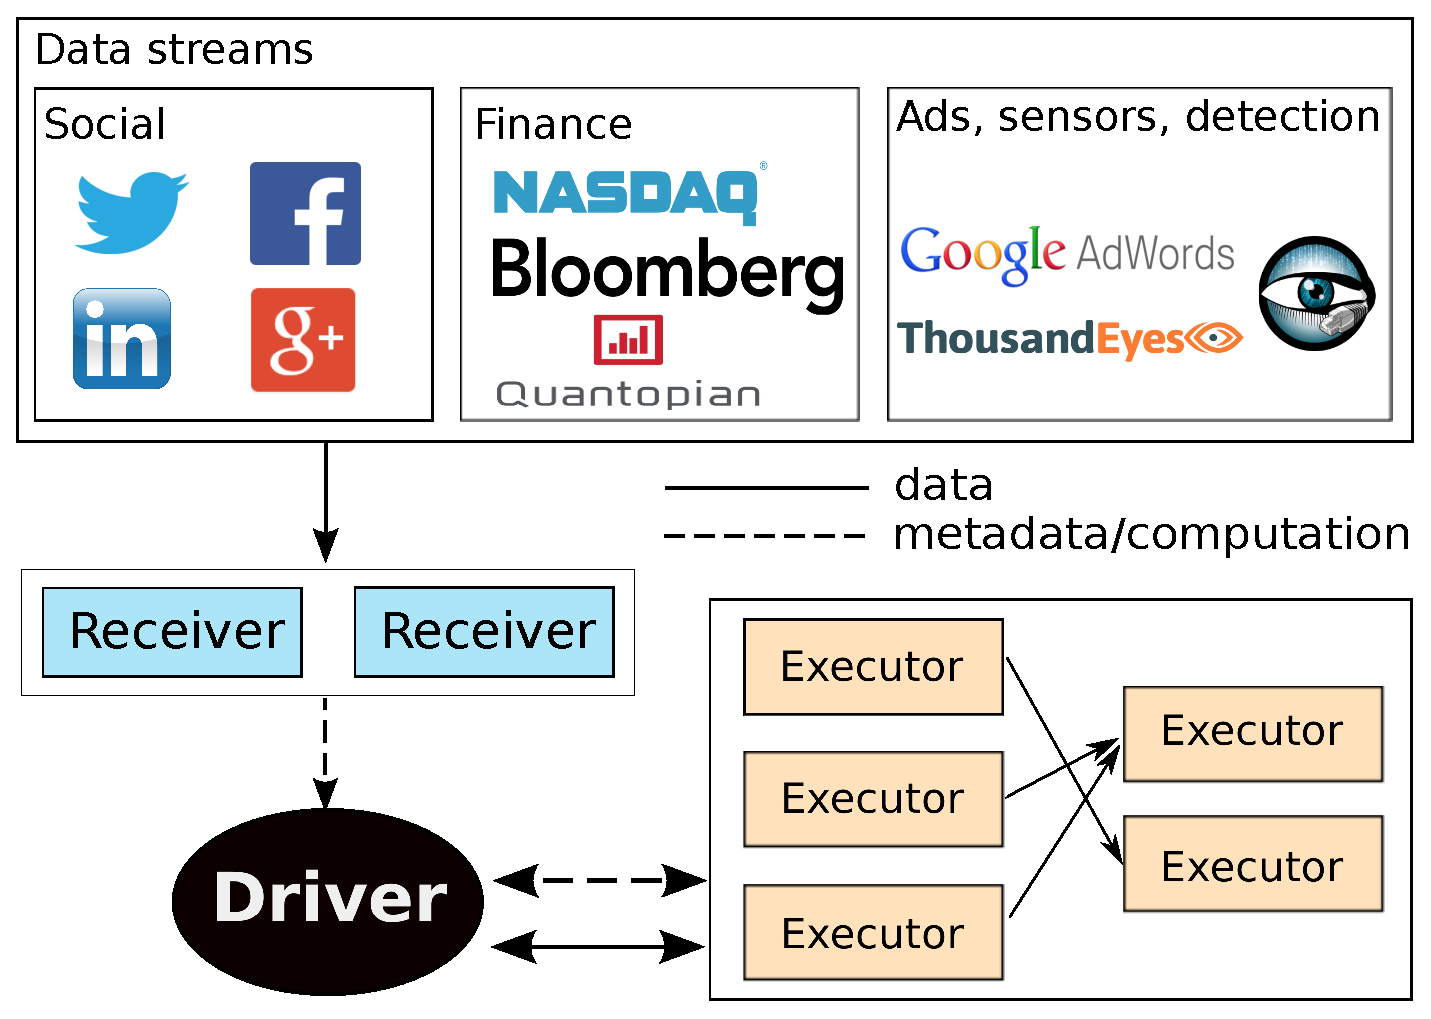
\includegraphics[scale=0.35]{images_graphs/spark_architecture_v4.eps}
  \end{center}
  \caption{Diagram of a Spark Streaming work flow. A Receiver and an Executor may execute in the same node.}
  \label{fig:SparkStreaming_architecture}
\end{figure}

In order to understand the rest of the paper we provide a short description of the architecture of Spark Streaming.

The execution of a Spark Streaming job works as depicted in Figure~\ref{fig:SparkStreaming_architecture}. 
First, data is generated at a source (e.g., tweets from Twitter). As the data is generated it is pushed to Spark Streaming, where it is received by a Receiver. 
The Receiver is responsible for receiving stream data and stash it in memory. Periodically, every <block interval> milliseconds, the Receiver takes the data stashed in memory and generates a block with that data. 
Once a block is generated, the Receiver informs a Spark Streaming's central component called Driver about this block. The Driver is responsible for holding metadata about the records received. 
Periodically, every <batch interval> milliseconds, the Driver takes the blocks that have been communicated by the receivers and that have not been processed yet and generates a batch job. 
Once this batch job is generated it is appended to a queue of jobs to be scheduled. 
The scheduler continuously polls this queue and schedules the jobs in the machines available in the cluster
Jobs are run in stateless isolated environments called Executors. Executors are usually deployed in the same nodes as Receivers.  \joao{is it always like this?}.

Internally, Spark Streaming makes extensive use of Actors -- a design pattern that decouples the invocation of methods from their execution. This means that 

For every Spark Streaming application, there is a driver and multiple executors. The receivers of data run on executors, and these receivers send to the driver metadata about the blocks generated. After every batch interval, the driver collects all of the blocks received during the period and make them into a RDD (Resilient Distributed Dataset, Spark's abstraction for distributed objects), and runs application logic on it using Spark. Spark runs each function on the RDD by generating tasks, serializing them, and sending them to appropriate executors. The executors deserialize each task, runs the function, and returns to the driver the results.
